%!TEX root = ../../main.tex
\section{Why Julia?}
\label{sec:Why Julia?}
The code for the algorithm presented in this chapter is all written in a recently released programming language called Julia.
Given that this language is still in beta version (it has yet to reach version 1 release) and is relatively unknown in the crystallography community, this choice may seem very unorthodox, so it is worth discussing why this was an adequate choice.

The total time of the implementation and run time of any piece of code can be crudely given as
\begin{equation*}
    \text{Total time} = \text{Computation time} + \text{Development time}
\end{equation*}
A compromise between the development time and the computation time has to be met, with the additional restraint that the developer's time is more important than the time of a computer.
Given that the development of a new algorithm requires lots of data and parameter exploration, writing prototype code in a low-level language such as C/C++ or Fortran would not necessarily be the optimum choice, particularly when the developer is unfamiliar with these languages.
A popular alternative is to use a high-level dynamic language such as Python, R or Matlab, which are usually designed, or have packages to support technical computing.
The productivity that can be achieved with these languages is counteracted by the relatively slow computation time when compared to low-level languages.

Julia is a dynamic language designed for technical computing \cite{bezanson2014julia,bezanson2012julia} that is also very fast.
Generally the computational performance of algorithms written in Julia run within a factor of 2 of the speed of C (Figure~\ref{fig:Language performance benchmarks}).
\begin{figure}[ht!]
    \centering
    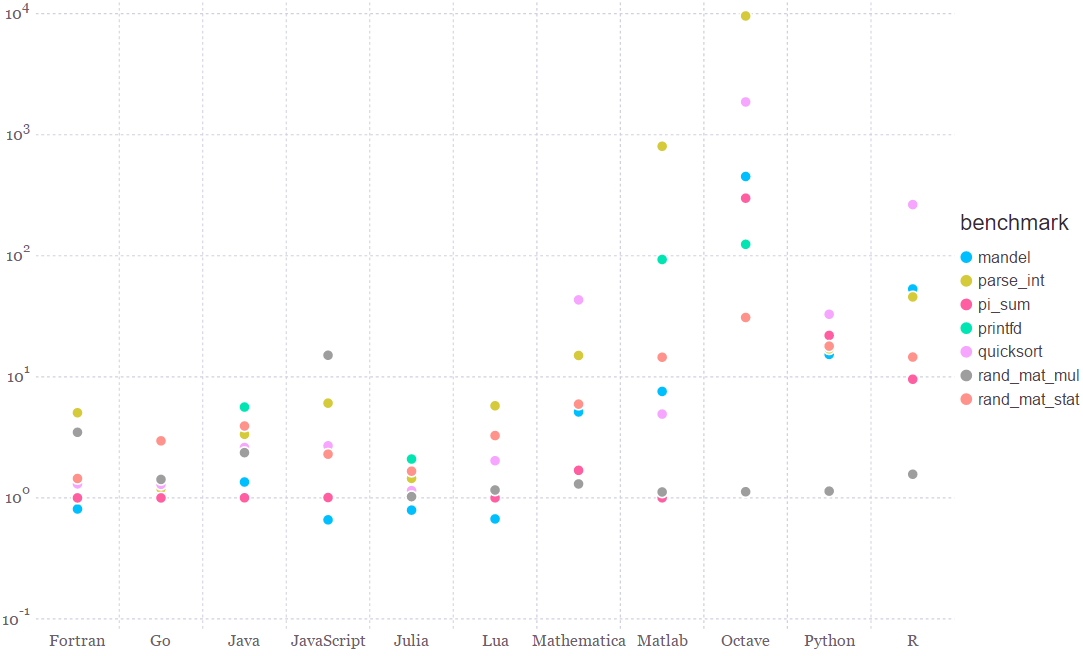
\includegraphics[width=1.0\textwidth]{figures/datared/language_benchmarks.png}
    \caption{Benchmark times taken to run a given algorithm for various languages relative to C (smaller is better, C performance = 1.0).
    The Python implementations of rand\_mat\_stat and rand\_mat\_mul use NumPy (v1.9.2) functions, the rest are pure Python implementations.
    The table of data for this plot can be found on the main Julia programming language webpage, \url{http://julialang.org/}, along with a link to the plot.}
    \label{fig:Language performance benchmarks}
\end{figure}
Therefore despite having to learn the Julia language, it seemed to be the best trade-off for the algorithm.

As a dynamic language that employs type inference, code can be written in Julia which may not be compiled to performance optimised machine code.
This means that Julia has to be written in a particular manner to achieve the performance claimed by the language authors.
A further argument for using Python or C/C++ over Julia is the large library of existing crystallographic packages that have been written in those languages.
However Julia has built-in support for calling methods from C/Fortran libraries with a single line of code.
Additionally the \verb+PyCall+ package was written in Julia to allow Python libraries to be accessed directly from Julia with a single line of code.
Therefore the crystallographic libraries were still easily accessible.

I expect that Julia and other languages that share a similar design (e.g. Go and Lua) will continue to increase in popularity over the years because of what they offer beyond their speed and ease.
All of Julia's packages are written in Julia because it is easy to write and it is fast.
This has greatly contributed to the fast growing Julia ecosystem.
This does not happen often with Python libraries like NumPy because to achieve performance, developers often have to resort to writing the performance critical parts in a low-level language like C.
This low barrier to creating useful packages is what Julia's real value is and it is the reason that I think we will see Julia grow in the years to come, particularly within the scientific community.
